\documentclass{article}
\usepackage[utf8]{inputenc}
\usepackage{amsmath}
\usepackage{amssymb}
\usepackage{amsthm}
\usepackage{cancel}
\usepackage[shortlabels]{enumitem}
\usepackage{caption}
\usepackage{graphicx}
\usepackage[top=0.5in, bottom=0.5in, left=1in, right=1in]{geometry}
\usepackage{float}

% \usepackage{titlesec}
%     \titlespacing{\subsection}{\parindent}{15pt}{12pt}

\title{\textbf{\underline{CSCI4030U: Big Data Analytics}\\Lab08}}
\author{Syed Naqvi\\100590852}
\date{\today}

\begin{document}

    \maketitle

    \subsection*{Ecoli Dataset}
    
    \begin{enumerate}[label = (\alph*), left=10pt, itemsep=10pt]
        
        \item \begin{minipage}[t]{0.9\textwidth}
            \textbf{C4.5 (weka.classifier.trees.J48)}\\
             Misclassification Rate: 15.7738\%\\
             Runtime: 0s
             \begin{figure}[H]
                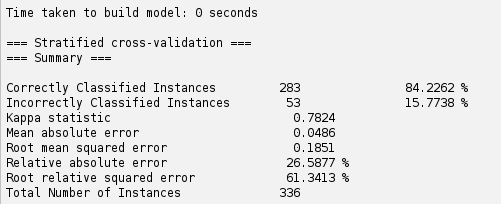
\includegraphics[width=0.75\textwidth, height=0.2\textheight]{./81a.png}
            \end{figure}
        \end{minipage}
        \item \begin{minipage}[t]{0.9\textwidth}
            \textbf{RIPPER (weka.classifier.rules.JRip)}\\
             Misclassification Rate: 19.3452\%\\
             Runtime: 0.03s
             \begin{figure}[H]
                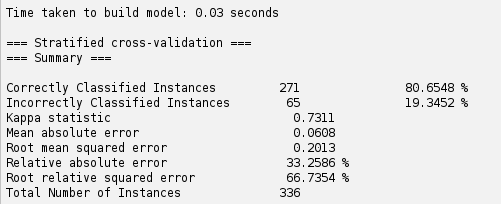
\includegraphics[width=0.75\textwidth, height=0.2\textheight]{./81b.png}
            \end{figure}
        \end{minipage}
        \item \begin{minipage}[t]{0.9\textwidth}
            \textbf{Naive Bayesian Classification (weka.classifiers.bayes.NaiveBayes)}\\
             Misclassification Rate: 14.5833\%\\
             Runtime: 0s
             \begin{figure}[H]
                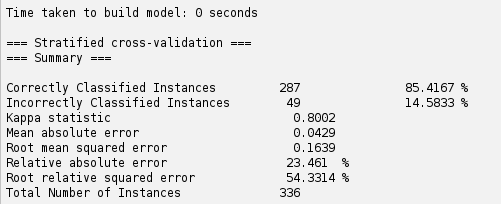
\includegraphics[width=0.75\textwidth, height=0.2\textheight]{./81c.png}
            \end{figure} 
        \end{minipage}
        \item \begin{minipage}[t]{0.9\textwidth}
            \textbf{k-Nearest Neighbor (weka.classifiers.lazy.IBk)}\\
             Misclassification Rate: 19.6429\%\\
             Runtime: 0s
             \begin{figure}[H]
                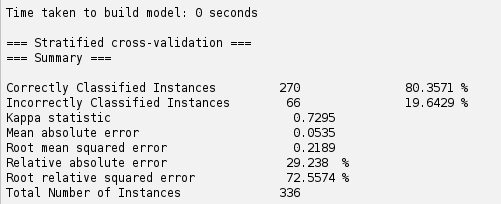
\includegraphics[width=0.75\textwidth, height=0.2\textheight]{./81d.png}
            \end{figure} 
        \end{minipage}
        \item \begin{minipage}[t]{0.9\textwidth}
            \textbf{Neural Networks (weka.classifiers.functions.MultilayerPerceptron)}\\
             Misclassification Rate: 13.9881\%\\
             Runtime: 0.3s
             \begin{figure}[H]
                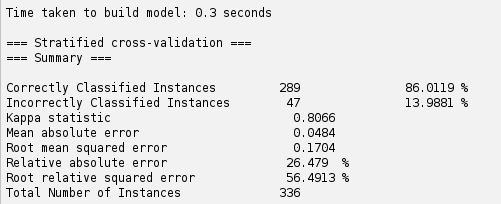
\includegraphics[width=0.75\textwidth, height=0.2\textheight]{./81e.png}
            \end{figure}
        \end{minipage}\\
        \vspace*{10pt}\\
        \begin{minipage}[t]{0.9\textwidth}
            The MultilayerPerceptron algorithm has the lowest misclassification rate but also had the highest runtime of 0.3 seconds. It is 
            likely context dependent if the incresed runtime costs are worth the improved accuracy. The k-nearest neighbor algorithm had the
            highest misclassification rate with a runtime of 0s while the RIPPER algoirithm had the second highest misclassification rate
            with a runtime of 0.03s.
        \end{minipage}
    \end{enumerate}

    \subsection*{Glass Dataset}
    
    \begin{enumerate}[label = (\alph*), left=10pt, itemsep=10pt]
        
        \item \begin{minipage}[t]{0.9\textwidth}
            \textbf{C4.5 (weka.classifier.trees.J48)}\\
             Misclassification Rate: 34.1121\%\\
             Runtime: 0s
             \begin{figure}[H]
                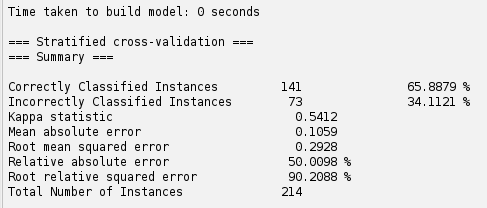
\includegraphics[width=0.75\textwidth, height=0.2\textheight]{./82a.png}
            \end{figure}
        \end{minipage}
        \item \begin{minipage}[t]{0.9\textwidth}
            \textbf{RIPPER (weka.classifier.rules.JRip)}\\
             Misclassification Rate: 30.3738\%\\
             Runtime: 0.01s
             \begin{figure}[H]
                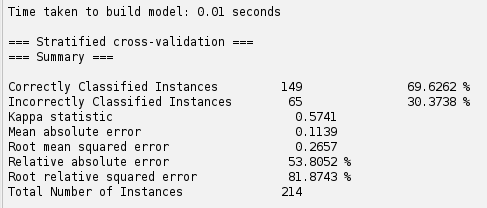
\includegraphics[width=0.75\textwidth, height=0.2\textheight]{./82b.png}
            \end{figure}
        \end{minipage}
        \item \begin{minipage}[t]{0.9\textwidth}
            \textbf{Naive Bayesian Classification (weka.classifiers.bayes.NaiveBayes)}\\
             Misclassification Rate: 50.4673\%\\
             Runtime: 0s
             \begin{figure}[H]
                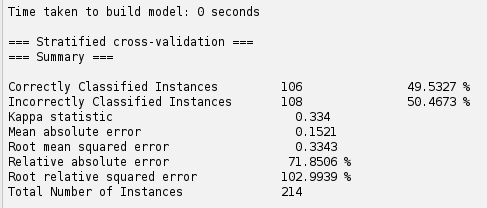
\includegraphics[width=0.75\textwidth, height=0.2\textheight]{./82c.png}
            \end{figure} 
        \end{minipage}
        \item \begin{minipage}[t]{0.9\textwidth}
            \textbf{k-Nearest Neighbor (weka.classifiers.lazy.IBk)}\\
             Misclassification Rate: 29.4393\%\\
             Runtime: 0s
             \begin{figure}[H]
                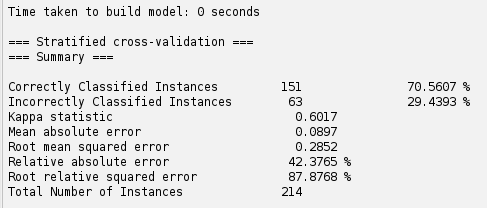
\includegraphics[width=0.75\textwidth, height=0.2\textheight]{./82d.png}
            \end{figure} 
        \end{minipage}
        \item \begin{minipage}[t]{0.9\textwidth}
            \textbf{Neural Networks (weka.classifiers.functions.MultilayerPerceptron)}\\
             Misclassification Rate: 30.8411\%\\
             Runtime: 0.3s
             \begin{figure}[H]
                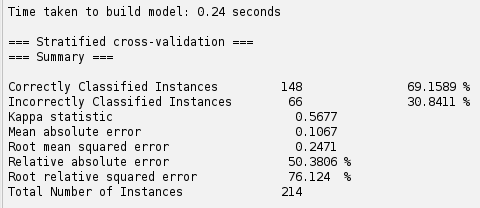
\includegraphics[width=0.75\textwidth, height=0.2\textheight]{./82e.png}
            \end{figure}
        \end{minipage}\\
        \vspace*{10pt}\\
        \begin{minipage}[t]{0.9\textwidth}
            For the Glass dataset there was a clear loser with the Naive Bayes algorithm. This algorithm had a misclassification rate
            of 50.4673\%. It seems that the classification rates for this dataset are lower in general with the k-nearest neighbors algorithm
            performing the best at 29.4393\% misclassification rate.
        \end{minipage}
    \end{enumerate}

    \subsection*{Image Dataset}
    
    \begin{enumerate}[label = (\alph*), left=10pt, itemsep=10pt]
        
        \item \begin{minipage}[t]{0.9\textwidth}
            \textbf{C4.5 (weka.classifier.trees.J48)}\\
             Misclassification Rate: 10.9524\%\\
             Runtime: 0.01s
             \begin{figure}[H]
                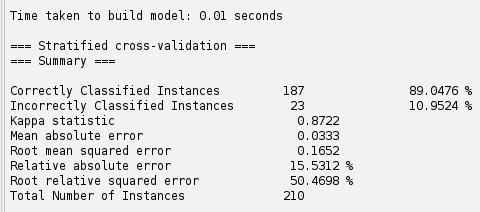
\includegraphics[width=0.75\textwidth, height=0.2\textheight]{./83a.png}
            \end{figure}
        \end{minipage}
        \item \begin{minipage}[t]{0.9\textwidth}
            \textbf{RIPPER (weka.classifier.rules.JRip)}\\
             Misclassification Rate: 20.4762\%\\
             Runtime: 0.01s
             \begin{figure}[H]
                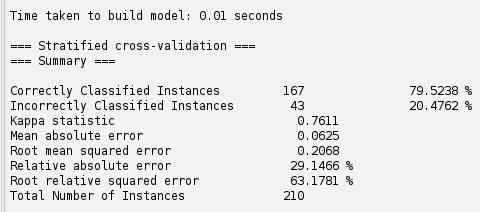
\includegraphics[width=0.75\textwidth, height=0.2\textheight]{./83b.png}
            \end{figure}
        \end{minipage}
        \item \begin{minipage}[t]{0.9\textwidth}
            \textbf{Naive Bayesian Classification (weka.classifiers.bayes.NaiveBayes)}\\
             Misclassification Rate: 22.381\%\\
             Runtime: 0s
             \begin{figure}[H]
                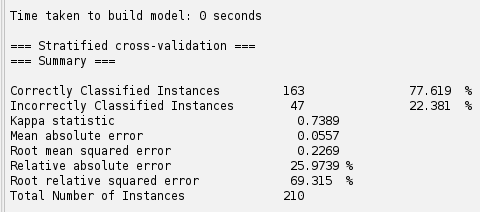
\includegraphics[width=0.75\textwidth, height=0.2\textheight]{./83c.png}
            \end{figure} 
        \end{minipage}
        \item \begin{minipage}[t]{0.9\textwidth}
            \textbf{k-Nearest Neighbor (weka.classifiers.lazy.IBk)}\\
             Misclassification Rate: 12.8571\%\\
             Runtime: 0s
             \begin{figure}[H]
                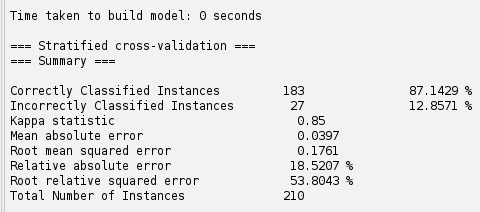
\includegraphics[width=0.75\textwidth, height=0.2\textheight]{./83d.png}
            \end{figure} 
        \end{minipage}
        \item \begin{minipage}[t]{0.9\textwidth}
            \textbf{Neural Networks (weka.classifiers.functions.MultilayerPerceptron)}\\
             Misclassification Rate: 11.4286\%\\
             Runtime: 0.45s
             \begin{figure}[H]
                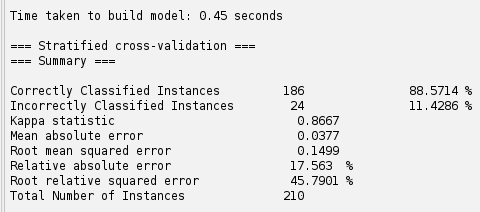
\includegraphics[width=0.75\textwidth, height=0.2\textheight]{./83e.png}
            \end{figure}
        \end{minipage}\\
        \vspace*{10pt}\\
        \begin{minipage}[t]{0.9\textwidth}
            For the image dataset there is larger variance in the misclassification rates acorss the various algorithms. The C4.5 algorithm
            has the lowest misclassification rate while the Naive Bayesian algorithm has the highest.
        \end{minipage}
    \end{enumerate}

    \begin{minipage}[t]{0.9\textwidth}
        \textbf{Conclusions:}\\
        Generally, the misclassification rates do not vary too much. It seems that the Neural Network algorithm consistenlty has the longest runtime
        while the c4.5 algoirithm is usually among the better performers. The closest thing to a clear loser would likely be the Naive Bayesian
        algorithm is it had the highest misclassification rates for both the Image and Glass datasets.
    \end{minipage}

\end{document}